%?????????????????????????
% Nombre: capitulo6.tex  
% 
% Texto del capitulo 6
%---------------------------------------------------

\chapter{Carga y pre-procesado de datos}
\label{limpieza-datos}

En este cap�tulo veremos las t�cnicas de tratamiento de datos utilizadas para la limpieza y refinamiento de un dataset que pueda ser usado para procesos posteriores como la visualizaci�n, el an�lisis de sentimientos y la obtenci�n de reglas de asociaci�n. Dado el volumen de los datos, y la naturaleza de los mismos, donde pr�cticamente cada uno de los 1.7M de tuits contiene alg�n elemento que hace que sea totalmente distinto de los dem�s, esta etapa fue una de las que m�s tiempo requiri�. 

\section{Carga de datos}

Una vez obtenidos y almacenados los datos en MongoDB, el siguiente paso l�gico del problema es pasarlos a RStudio, donde por medio de nuestros scripts comenzar�amos con el tratamiento de los mismos. Es en este punto, donde topamos con el primer problema que nos lleva a un enfoque basado en Big Data del problema dado que ninguna de las herramientas nativas de R ni las conexiones directas de R con MongoDB de paquetes como \textit{rmongodb} pueden manejar el dataset completo para obtener 1.7M  de documentos almacenados en MongoDB y pasar su contenido a un tipo de dato \textit{data-frame} de R. 

La soluci�n, la encontramos en el paquete \textbf{\textit{SparkR}}. Este paquete \cite{sparkr}, crea una sesi�n distribuida por medio de virtualizaci�n (figura \ref{sparkrdis}) en Spark que ofrece funciones de filtrado, agregaci�n y selecci�n entre otras muchas, de manera similar a como se podr�a hacer con los dataframes nativos de R, con la diferencia de que al ser desde un enfoque distribuido, hace uso de unos objetos denominados, \textit{SparkDataFrames}. Estos objetos, pueden manejar grandes colecciones de datos ya que los distribuyen en columnas, que pueden ser construidas como en nuestro caso con una base de datos noSQL externa, aunque hay otras t�cnicas viables.

\begin{figure}[h]
\centering
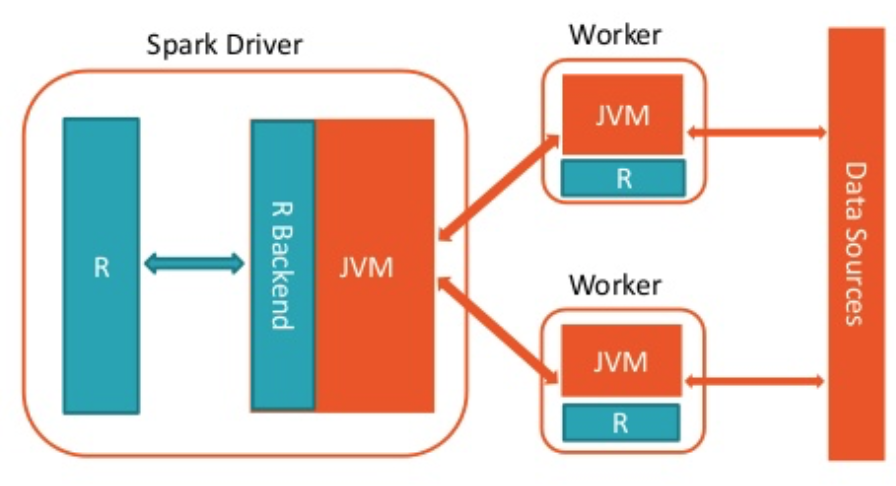
\includegraphics[width=7cm]{./Capitulo6/imagenes/arq.png}
\caption{Arquitectura de Spark R.}
\label{sparkrdis}
\end{figure}

Una vez obtenidos los datos, en nuestra sesi�n de Spark en RStudio, debemos pasarlos a la sesi�n b�sica de R. Esto es as� debido a que  Rstudio es el anfitri�n de Spark, pero las sesiones difieren, por lo que debemos operar entre ambas por medio de funciones b�sicas de Big Data como \textit{collect} para el caso que nos compete de fusionar nuestro SparkDataFrame a un DataFrame de R. 

\section{Pre-procesado}



\pagebreak
\clearpage
%---------------------------------------------------